\section{\label{sec:clas.cc}\texorpdfstring{\v{C}}{C}erenkov Counters (\abbr{CC})}

The \emph{gas} \v{C}erenkov counters (\abbr{CC}), indicated in Fig.~\ref{fig:clas}, occupies the space between the drift-chambers and the time-of-flight counters in each of the six sectors. They are divided into 18 segments (shown in Fig.~\ref{fig:clas.cc}) in the polar angle, $\theta$, away from the beam line. These segments are designed to focus \v{C}erenkov-light emitted from particles originating from the center of \abbr{CLAS}. The coverage in $\theta$ is approximately 8$^\circ$ to 45$^\circ$ for tracks originating from the center of \abbr{CLAS}. Because the target was placed 90~cm upstream, the polar coverage was in the range from 6$^\circ$ to 35$^\circ$ in the lab frame.

\begin{figure}\begin{center}
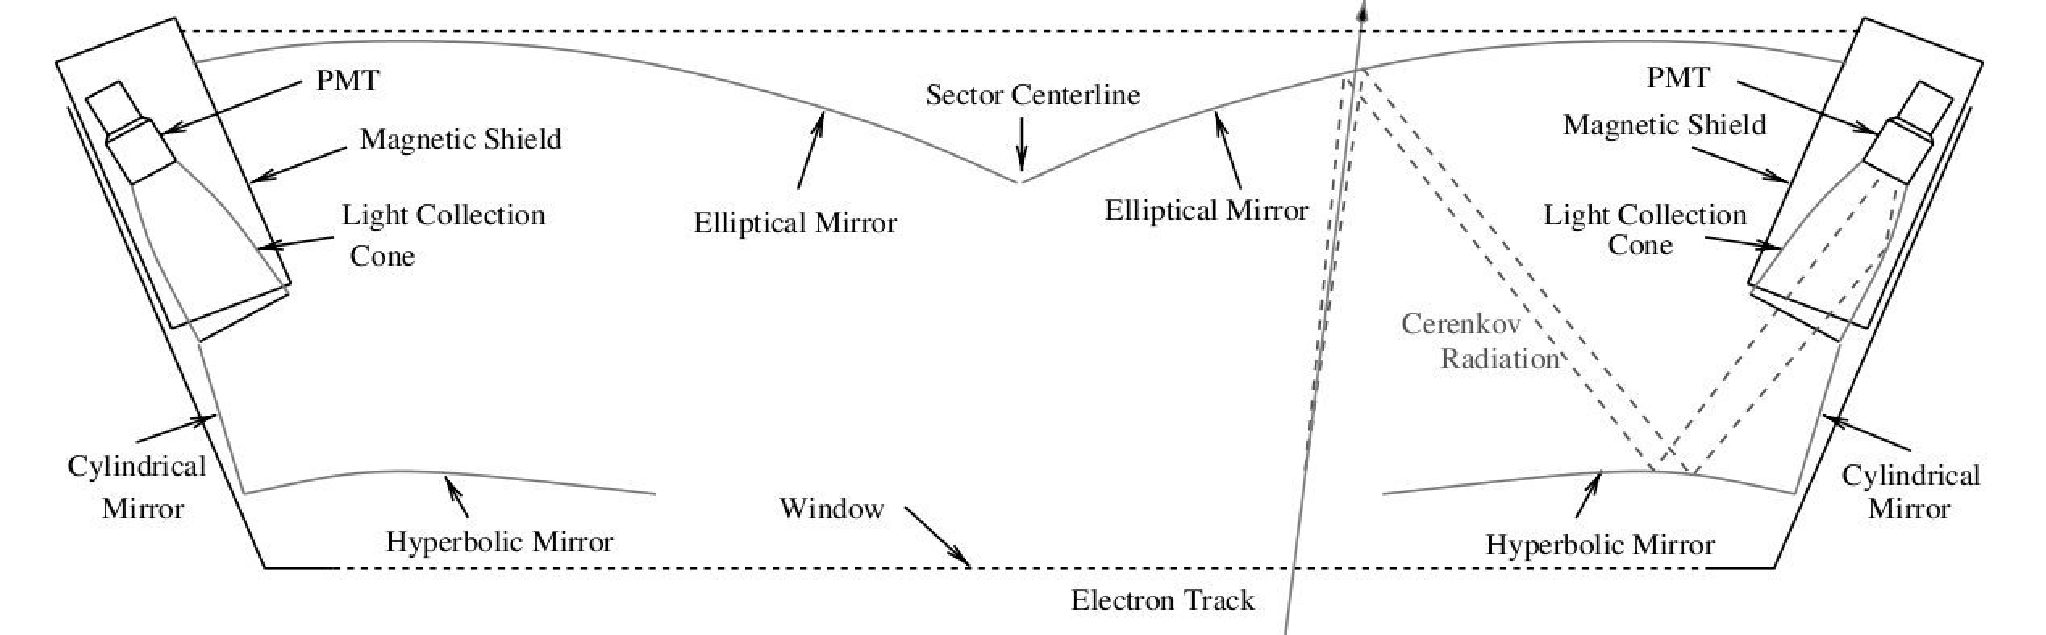
\includegraphics[width=0.9\columnwidth]{\figures/hall-b/cc_diagram.pdf}
\caption[\v{C}erenkov Detector Segment Diagram]{\label{fig:clas.cc}Diagram of one segment of the \v{C}erenkov counters with an electron entering from the bottom.}
\end{center}\end{figure}

The gas used in the \abbr{CC} is perfluorobutane (C$_4$F$_{10}$) with an index of refraction of 1.00153. The charged pion threshold for this detector is approximately 2.7~GeV, while the threshold for electrons is 9~MeV. Thresholds for kaons and protons are much higher than the maximum beam energy for \g12 and were therefore not detected in the \abbr{CC}. The detecting efficiency for electrons is $> 97\%$ and this detector enabled the distiction between pions and electrons below approximately 2.5~GeV.

The use of the \abbr{CC} was not included in the original proposals, however a significant drop in price on C$_4$F$_{10}$ just prior to the start of \g12 allowed the gas to be added at the last minute. The price drop was due to the recent availability of another, much cheaper gas that was demonstrated to have the same general properties as C$_4$F$_{10}$.

\begin{figure}\begin{center}
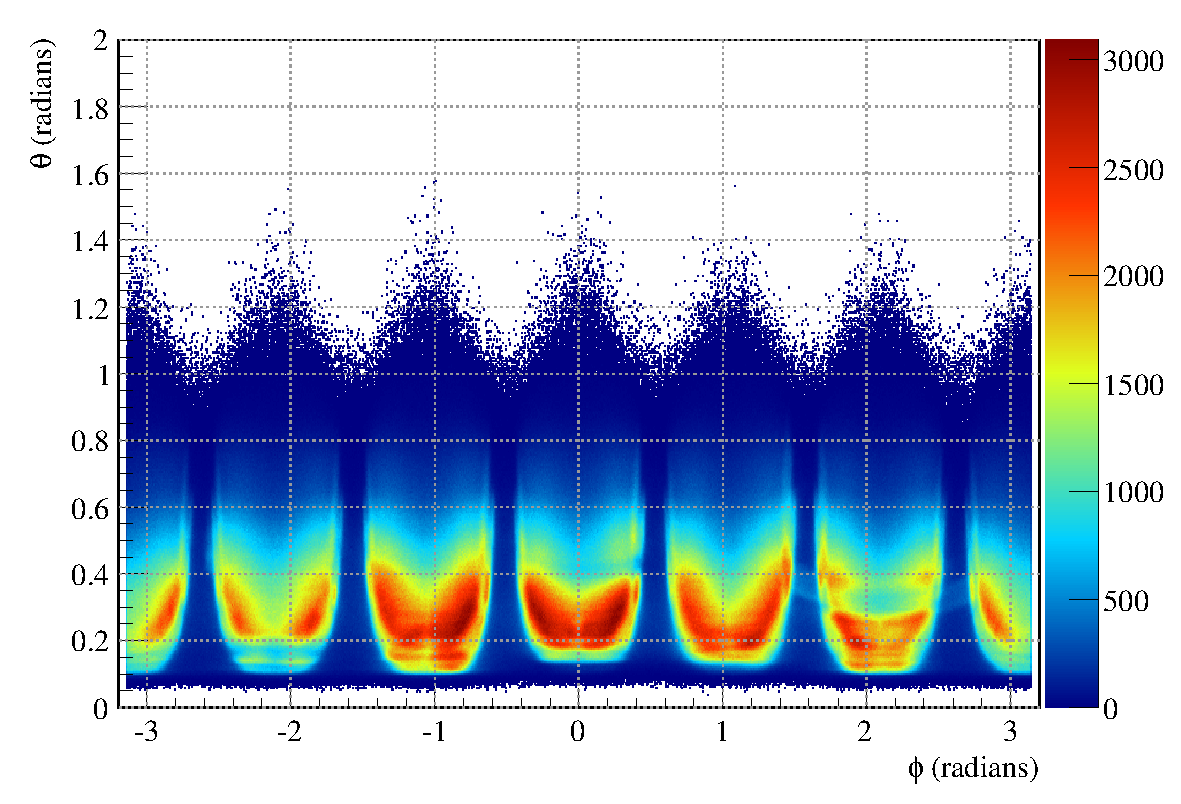
\includegraphics[width=\figwidth]{\figures/reconstruction/coverage_cc.pdf}
\caption[\v{C}erenkov Counter Angular Coverage]{\label{fig:clas.cc.coverage}{\coloronline}Angular coverage in the lab frame of the tracks that had an associated \v{C}erenkov counter hit.}
\end{center}\end{figure}
